\documentclass[thesis.tex]{subfiles}

\begin{document}
\ifSubfilesClassLoaded{

% \section{Definitions}
% \todo[inline]{These will be defined in the introductory chapters, but are here so that this draft is understandable}
% \begin{itemize}
% \item
%   We assume that, for all episodes $i$, $D_i$ is iid and independent
%   of the time of the infection. Define the survival function
%   $\prob(D_i \geq t \mid B_{j(i)} = b, \theta) = \prob(D_i \geq t \mid \theta) = S_\theta(t)$,
%   where $\theta$ are the parameters controlling the survival
%   distribution (the discussion in this document is valid regardless of
%   the model specified for $S_\theta$ and hence we consider $\theta$
%   as an arbitrary vector of parameters).
% \item
%   The beginning of episode $i$ is known to occur in the interval
%   $[l_{j(i)}^{(b)}, r_{j(i)}^{(b)}]$, and similarly for the end of the infection
%   in $[l_{j(i)}^{(e)}, r_{j(i)}^{(e)}]$.
% \end{itemize}

\setcounter{chapter}{4}
}

\chapter{Estimating duration with infrequent testing} \label{perf-test}

When estimating incidence from prevalence, the mean duration, not its median, is the most important feature of the duration distribution~\autocite{freemanPrevalence}.
Duration distributions tend to be right-skewed.
Therefore, estimates of the mean are sensitive to the tail of the duration distribution.

In \cref{E-ATACCC} I estimated the duration distribution from the ATACCC dataset.
However, this study suffered from a small sample size and only 20 days of follow-up, enabling estimation of the tail.
Therefore, model assumptions drive the size of the estimated tail.

In this chapter, I develop a method to estimate the duration distribution using CIS data.
The CIS sampling is less frequent, but with a large sample size and long follow-up.

I take a Bayesian survival analysis approach to model the coarse sampling of the CIS (\cref{perf-test:sec:problem}).
I use a simulation study (\cref{perf-test:sec:simulation-study}) to evaluate a range of priors for the survival distribution (\cref{perf-test:sec:parameters-priors}).
These include a prior to combine the information in the CIS with the results of \cref{E-ATACCC}.
Reasonable priors successfully recover the true distribution.
However, the method must be able to account for false negatives, discussed in \cref{E-imperf-test}.

\section{Problem description} \label{perf-test:sec:problem}

The CIS tests each individual infrequently, either weekly or monthly (see \cref{E-intro:sec:cis}).
The infrequent testing complicates analysis of the data in two ways.
First, infection episodes can go undetected.
Second, the infection episode start and end times are known imprecisely.
This section explains these issues. The rest of the chapter develops a method to tackle  them.

\subsection{Undetected infections}

The first complication in the analysis is that infection episodes can be undetected.
Undetected infection episodes are episodes with no associated positive tests.
Therefore, there is no information directly observed about the episode; even the number that occur is unobserved.
They occur when an episode starts and ends between tests (see \cref{perf-test:fig:truncation}).
Undetected episodes are important because they are shorter than detected episodes.
To see why this is the case, consider the undetected infection in the bottom of \cref{perf-test:fig:truncation}.
The infection episode depicted begins at time 33 and has a 10-day duration.
If the duration had been 24 days or more, the individual would still be detectable at their next test and detected then.
CIS has many undetected infections.
This is because the interval between tests in the same individual (up to 28 days, see \cref{E-intro:sec:cis}) is longer than most infections (median 16 days, see \cref{E-ATACCC:sec:results}).
\begin{figure}
  \makebox[\textwidth][c]{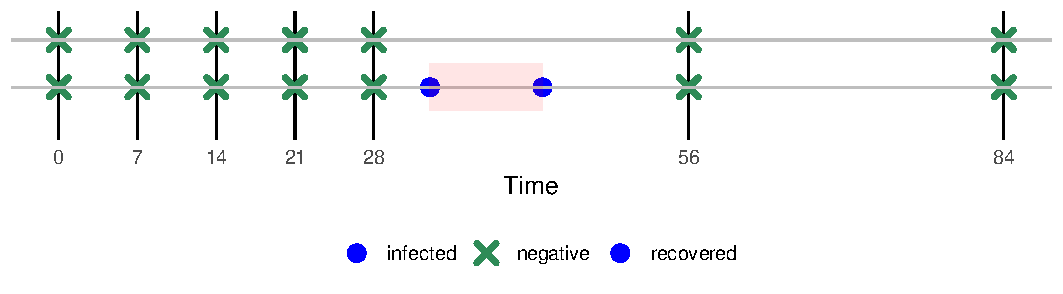
\includegraphics[width=1.2\textwidth]{cis-perfect-testing/truncation}}
  \caption[Undetected episodes in CIS data]{An unknown number of infection episodes in CIS are undetected. Consider the two individuals shown here: we collect identical data for them (a series of negative tests) yet the top individual was never infected and the bottom individual was. See the main text for why this is an issue. \label{perf-test:fig:truncation}}
\end{figure}

\subsection{Unobserved episode beginning and end times} \label{perf-test:sec:interval-censoring}

The second complication is that the exact beginning and end times of detected infection episodes are unknown.
The imprecision in the beginning of the infection episode arises because the only observation that episode $j$ has started is that an individual was negative at one test, on day $l_j^{(b)}-1$ (the minus one is because the first day that the infection could have begun is the day after the negative test), and positive at the next test, on day $r_j^{(b)}$.
Similarly, the end of the infection episode is bounded by the final positive test on day $l_j^{(e)}$ and the following negative test on day $r_j^{(e)}+1$ (the plus one is because the last day that the infection could have ended is the day before the negative test).
\Cref{perf-test:fig:double-interval-censor} shows this issue graphically.
\begin{figure}
  \centering 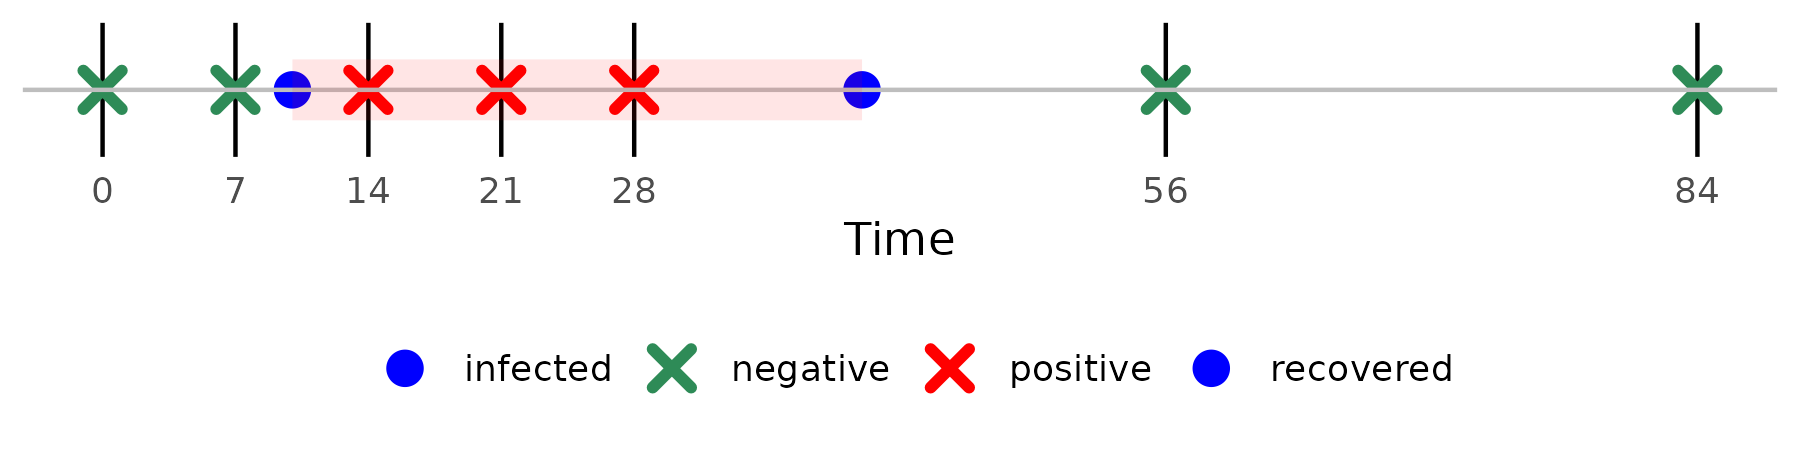
\includegraphics{cis-perfect-testing/double-interval-censor}
  \caption[Double-interval censoring in CIS data]{Episodes data in CIS is double interval censored, meaning that both the start and end of the episode are only known up to an interval. Demonstrated here by a participant who is recorded negative at time 7 to positive at time 14, bounding the start of the episode; similarly, changing from positive at time 28 to negative at time 56 bounds the end of the episode. \label{perf-test:fig:double-interval-censor}}
\end{figure}

\subsection{Approach} \label{perf-test:sec:approach}

I base my analysis on the 4,800 episodes that were first detected between 10th Oct 2020 and 6th Dec 2020 inclusive with negatives bounding the start and end time of the episode.
That is, the individual tested negative before and after the episode.
Without a negative before the episode there is no lower bound on the episode's start time.
It could be arbitrarily long and there is little information on its length.
A negative test follows each episode unless the individual was lost to follow-up before their episode ended.
This is rare.
Episodes removed in this step are incorporated in the adjustment for undetected episodes.

\section{Survival analysis}

In survival analysis, the event at the start of the time of interest is the \emph{initiating event}, and the event at the end of the time of interest is the \emph{terminating event}.
It is used in many areas, including how long a machine lasts before breaking down or how long a patient spends in hospital after a treatment.
Here, I am estimating the distribution of the duration of positivity.
The initiating event is the episode's start; the terminating event is the episode's end.

Undetected events where there is no information on these events is known as \emph{truncation}.
A situation that is particularly relevant is \emph{left truncation}, when only events lasting a minimum amount of time are observed.
There is a subtlety that makes the CIS different from standard left truncation.
In CIS, individuals in which undetected infections occurred are enrolled in the study.
Therefore, some data has been collected about them.
In standard left truncation, nothing is known about the missed events.
Here, I will incorporate the additional information into the analysis.
I refer to these events as ``undetected'', rather than truncated, to emphasise this difference.

The time of the initiating and/or terminating events are not known exactly.
This is known as \emph{censored} in the survival analysis literature.
Censored events are present in almost all survival analyses.
An event is \emph{left censored} if it is known to occur before a certain time.
An event is \emph{right censored} if it is known to occur after a certain time.
An event is \emph{interval censored} if it is known to occur within an interval.
%Left and right censoring can be viewed as special cases of interval censoring where the lower bound is negative infinity or the upper bound is positive infinity respectively.
As explained in \cref{perf-test:sec:problem}, the initiating and terminating events are only bounded, and hence interval censored.
The data is \emph{doubly censored} because both the initiating and terminating events are censored.
To handle doubly censored data, the times need to be jointly modelled~\autocite[and references therein]{liSemiparametric}.
In CIS data both the initiating and the terminating events are interval censored.
Therefore, the CIS data is \emph{double interval censored}.
\Textcite{sunAnalysis,bogaertsSurvival} review methods for double interval censored data.

Few studies look at the combination of both double interval censoring and undetected (or truncated) events.
This is especially true within the human biostatistical literature.
The literature does include theoretical frameworks which include the double censored and truncated case~\autocite{turnbullEmpirical,dempsterMaximum}, yet these frameworks have only been applied when the terminating event was either uncensored or right censored~\autocite{sunEmpirical,bacchettiNonparametric}.
These studies \autocite[and elsewhere, e.g.:][]{shenNonparametric} take a conditional likelihood approach.
They condition on the truncation (a selection effect) and the period where the initiating event occurs.
They condition on the initiating event time because it provides negligible information on the distribution of interest~\citePersonalComms{Nick Jewell}.
This is not the case for the CIS.
In CIS, infection episodes are more likely to be detected when an individual is in the weekly testing phase.
Therefore, the probability of an infection episode being detected conditional on being infected is higher than the overall probability of being detected.

Censored and truncated data are normal for estimation of the survival time of bird and insect nests~\autocite{heiseyABCs}.
\textcite{heiseyModelling} developed a framework for handling this situation.
The framework is general, allowing for arbitrary censoring patterns and double interval censoring.
They apply it to a situation the visit times are global (all nests could be detected on the same days), simplifying the likelihood.
I adapt this framework for CIS, when each individual has their own visit schedule (see section \cref{perf-test:sec:model}).

I use Bayesian inference for two reasons.
First, frequentist estimators are poorly developed and their properties (\eg consistency and convergence rate) are poorly understood~\autocite{sunAnalysis,dengNonparametric}.
Second, a prior can include information from previous studies, such as from \cref{E-ATACCC}.
Alternatively, the prior can favour a smoothly changing hazard.
I explore priors in section 1.4.
These prior structures overcome issues caused by the undetected episodes ~\autocite{caoBias}.

Bayesian methods have been used for nest survival before~\autocite{heBayesiana,heBayesian,caoModeling} by augmenting the data with the unobserved times of infection.
The augmentation creates a parameter per detected infection.
This increases the dimensionality of the problem greatly, making it computationally infeasible within the SRS.
I develop a novel Bayesian framework without explicit data augmentation.
This method scales to the large number of episodes present in CIS.


\section{Modelling the duration}\label{perf-test:sec:model}

In this section, I develop a model accounting for double interval censoring and undetected episodes.
This approach extends the framework of \textcite{heiseyModelling} to include individuals without detected episodes.
This framework is itself based long-standing methodology~\autocite{dempsterMaximum,turnbullEmpirical}.
I augment the data set with the full number of episodes, including those that are undetected.

Integrating over the number of missed episodes is possible analytically.
This makes inference tractable within modern, high-performance Bayesian software such as Stan.
Let the total number of infection episodes in the cohort be $\ntot = \ndet + \nnodet$ where $\ndet$ is the number of detected infections and $\nnodet$ is the number of undetected infections.
Let $\Ncis$ be the number of individuals in the cohort and $\nsched$ be the number of test schedules.
%Without loss of generality, let the individuals with a detected episode be indexed by $i = 1, \dots, \ndet$ and the individuals without a detected episode be indexed by $i = \ndet + 1, \dots, \Ncis$.
Let $i = 1, \dots, \nsched$ index infection schedules and $j = 1, \dots \ntot$ index infection episodes.

All the relevant information about episode $i$ can be fully characterised by the (unobserved) triplet $(b_j, e_j, \sched_j)$ where $b_j$ and $e_j$ are the times the episode being and end respectively and $\sched_j$ is the set of test times for the individual in which the episode occurs.
The episode's duration is $d_j = e_j - b_j + 1$.
%, the number of days the individual in which the episode occurred, was positive for 
This triplet is assumed iid.

$b_j$ and $e_j$ span possible infection and recovery times.
$\sched_j$ is one of the observed test schedules, with any other test schedule assumed to occur with probability zero.
Over the short period of time considered, each unique test schedule has zero or one detected episodes.

Let $i \in \set{D}$ indicate $\sched_i$ is associated with a detected episode.
That is, $i \in \set{D}$ if and only if there exists a $j(i)$ such that $b_{j(i)}$ and $e_{j(i)}$ such that $(b_{j(i)}, e_{j(i)}, \sched_i)$ is a detected episode.
$(b_{j(i)}, e_{j(i)}, \sched_i)$ is a detected episode when the following three conditions are met.
First, $\exists t \in \sched_i$ such that $b_{j(i)} \leq t \leq e_{j(i)}$; this condition is equivalent to having at least one positive test for the episode.
Second, $\exists t \in \sched_i$ such that $t < b_{j(i)}$, to lower bound the start of the episode.
Finally, $\exists t \in \sched_i$ such that $t > e_{j(i)}$, to upper bound the end of the episode; this condition will be met for any episode sufficiently far in the past in individuals not lost to follow-up (almost always the case in this context).
For a new context where recent infections need to be considered, this condition can be relaxed by considering these episodes as right-censored, at little cost except a more complicated likelihood expression.


To relate the state space to the data, I define three subsets partitioning the space of possible infection and recovery times (\ie: are strict subsets of $T \times T$), for a test schedule $\sched_i$.
Figure \ref{perf-test:fig:partitionSpace} shows this graphically.
Each episode, whether detected or not, must fall into one of these three classes with a probability that is a function of the model parameters, $\theta$.

\begin{itemize}
\item
  Admissible episodes, $\alpha_i$, which have an infection and recovery time consistent with the data observed.
  This space is empty for $i \notin \set{D}$; in this case, $n_{ia} = 0$ admissible episodes occurred in individuals with test schedule $\sched_i$.
  Otherwise, $i \in \set{D}$ then $n_{ia} =1$ admissible episode occurred in an individual with test schedule $\sched_{i}$.
  Conditional on the episode occurring in individuals with test schedule $\sched_i$, it is admissible with probability $p_{ia} = \prob((b, e) \in \alpha_i \mid \theta)$.
  \label{perf-test:def:admissible}
\item
  Undetected episodes, $\Omega_i^C$, which have an infection and recovery time such that they would not have tested positive.
  An unknown number, $n_{iu}$ of these observed in individuals with test schedule $\sched_i$.
  Conditional on the episode occurring in individuals with test schedule $\sched_i$, it is undetected with probability $p_{iu} = \prob((b, e) \in \Omega^C_i \mid \theta)$.
\item
  Inadmissible episodes, $\beta_i$, which are not consistent with the data observed but would have been
  detected.
  This is all remaining episodes not in the previous sets.
  $n_{i\bar{a}} = 0$ of these occurred in any individuals with test schedule $\sched_i$.
  Conditional on the episode occurring in these individuals, it is inadmissible with probability $p_{i\bar{a}} = \prob((b, e) \in \beta_i \mid \theta)$.
\end{itemize}

% The detected region, $\Omega_i = \alpha_i \cup \beta_i$, for test schedule $\sched_i$ is the region where we could have observed episodes. 
% The notation is for consistency with \textcite{heiseyModelling}.
% $\Omega_i$ is the complement of $\Omega^C_i$.

\begin{figure}
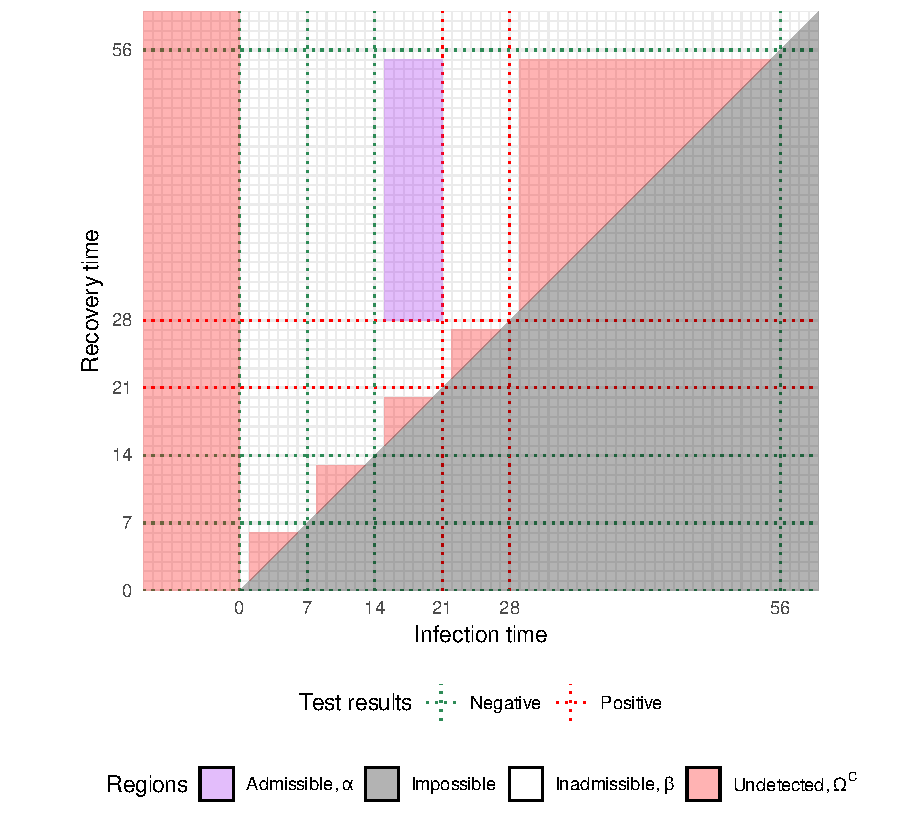
\includegraphics[width=\textwidth]{cis-perfect-testing/regions_diag}
\caption[Admissible, inadmissible, and undetected infections]{The regions (as defined in the main text) for an individual with test schedule $\sched_i$ whose first test was at time 0 and negative, with subsequent
negative tests at times 7, 14, and 56, and positive tests at times 21
and 28. Inadmissible region is unshaded. The black (impossible) region is because it does not make sense for recovery to occur prior to infection. \label{perf-test:fig:partitionSpace}}
\end{figure}

These three classes span all possible episodes and are mutually exclusive.
Hence, $\ntot = \ndet + \nnodet + n_{i\bar{a}} = \sum_{i=1}^{\nsched} n_{ia} + \sum_{i=1}^{\nsched} n_{iu} + 0$.
Furthermore, for all $i$, $p_{ia} + p_{iu} + p_{i\bar{a}} = 1$.

Any episode $j$ independently belongs to one of these classes.
I assume the individual in which each episode occurs is iid uniform across the cohort.
Therefore, conditional on $\ntot$, the number of episodes in each class, $(n_{ia}, n_{iu}, n_{i\bar{a}})^T$, are distributed multinomially.
The above probabilities ($p_{iu}$, $p_{ia}$, and $p_{i\bar{a}}$) are conditional on the episode occurring with test schedule $\sched_i$.
These probabilities are multiplied by $\eta_i/\Ncis$, where $\eta_i$ is the number of individuals with test schedule $\sched_i$, to give the probability that an episode belongs to each class, without conditioning on a specific individual.

The undetected classes for each individual cannot be distinguished by any observable data.
Each class's count needs to be marginalised over to calculate the likelihood.
Because the counts have a joint multinomial distribution, this is equivalent to only considering the sum of the counts.
The overall probability of an episode being unobserved is $\pnodet = \frac{1}{\Ncis} \sum_{i=1}^{\nsched} \eta_i p_{iu}$.
Furthermore, the inadmissible classes are guaranteed to have zero episodes.
Counts of zero do not contribute to a multinomial pmf (they multiply by 1).
Therefore, I combine the undetected classes into a single class and ignore the inadmissible classes.

Let $\na = (n_{1a}, \dots, n_{\nsched a})^T$ be the vector of counts of episodes in the admissible classes.
The counts $\na$ and $\nnodet$ are jointly distributed multinomially.
The support of the distribution requires $\nnodet = \ntot - \sum_{i=1}^{\nsched} n_{ia} = \ntot - \ndet$ and $\ntot \geq \ndet$.
Hence:
\begin{align}
p(\na \mid \ntot, \theta)
&= p(\nnodet, \na\mid \ntot, \theta) \\
&= \frac{\ntot!}{\nnodet! \prod_{i=1}^{\nsched} n_{ia}!}  \pnodet^{\nnodet}\prod_{i=1}^{\nsched} \left(\frac{1}{\nsched}p_{ia}\right)^{n_{ia}} \\
&\propto \frac{\ntot!}{(\ntot - \ndet)!} \pnodet^{\ntot - \ndet} \prod_{i \in \set{D}} p_{ia} \label{perf-test:eq:augmented-likelihood}
\end{align}
the final line follows because $\nnodet = \ntot - \ndet$, $n_{ia} = 1$ for $i \in \set{D}$, and $n_{ia} = 0$ otherwise.

In forming the probability $p_{ia}$, the data is used.
This is not quite correct because the cell probabilities in the likelihood should not depend on the data.
However, an alternative where each combination of infection and recovery times is considered its own class is possible.
Then, the counts for all the classes that previously contained undetected episodes would be zero.
The resulting likelihood would be the same.
Therefore, I present this version as it is clearer.

The posterior density we are interested in is $p(\theta \mid \na)$.
It can be written as follows.
\begin{align}
p(\theta \mid \na)
&\propto p(\theta) p(\na \mid \theta) \\
&= p(\theta) \sum_{\ntot=\ndet}^\infty p(\ntot \mid \theta) p(\na \mid \theta, \ntot) \\
&\propto p(\theta) \sum_{\ntot=\ndet}^\infty \left( p(\ntot \mid \theta) \frac{\ntot!}{(\ntot - \ndet)!} \pnodet^{\ntot - \ndet} \prod_{i \in \set{D}} p_{ia} \right) \\
&= p(\theta) \left( \prod_{i \in \set{D}} p_{ia} \right) \left( \sum_{\ntot=\ndet}^\infty p(\ntot \mid \theta) \frac{\ntot!}{(\ntot - \ndet)!} \pnodet^{\ntot - \ndet} \right) \label{perf-test:eq:full-posterior}.
\end{align}
The rest of this section derives expressions for each $p_{ia}$, $p_{u}$ and the sum.

To start, I derive an analytical solution to $\sum_{\ntot=\ndet}^\infty p(\ntot \mid \theta) \frac{\ntot!}{(\ntot - \ndet)!} \pnodet^{\ntot - \ndet}$ under the prior $\ntot \dist \NBc(\mu, r)$.
I assume that $\theta$, which are only the parameters of the survival distribution, has a prior independent of $\ntot$, the number of infections that occurred in the cohort.
Therefore, $p(\ntot \mid \theta) = p(\ntot)$.
Putting a negative binomial prior on $\ntot$ is equivalent to the following gamma-Poisson composite; its use simplifies the derivation.
\begin{align}
\ntot \mid \lambda &\dist \Poi(\lambda) \\
\lambda &\dist \GamDist(a, b)
\end{align}
where $b = r / \mu$ and $a = r$.
Hence:
\begin{align}
&\sum_{\ntot=\ndet}^\infty \frac{\ntot!}{(\ntot-\ndet)!} \pnodet^{\ntot-\ndet} p(\ntot) \\
&= \int \sum_{\ntot=\ndet}^\infty \frac{\ntot!}{(\ntot-\ndet)!} \pnodet^{\ntot-\ndet} p(\ntot \mid \lambda) p(\lambda) d\lambda &\text{$\lambda$ explicit}\\
&= \int \sum_{\ntot=\ndet}^\infty \frac{\ntot!}{(\ntot-\ndet)!} \pnodet^{\ntot-\ndet} \frac{\lambda^{\ntot} e^{-\lambda}}{\ntot!} p(\lambda) d\lambda &\ntot \dist \Poi\\
%&= \int \sum_{\ntot=\ndet}^\infty \frac{1}{(\ntot-\ndet)!} \pnodet^{\ntot-\ndet} \lambda^{\ntot-\ndet} \lambda^{\ndet} e^{-\lambda} p(\lambda) d\lambda \\
&= \int \lambda^{\ndet} e^{-\lambda} p(\lambda) \sum_{\nnodet=0}^\infty \frac{(\pnodet \lambda)^{\nnodet}}{\nnodet!} d\lambda &\nnodet = \ntot-\ndet\\
&= \int \lambda^{\ndet} e^{-\lambda} p(\lambda) e^{\lambda \pnodet} d\lambda &\text{Maclaurin series of $e$} \\
&= \int \lambda^{\ndet} e^{-\lambda(1 - \pnodet)} \frac{b^a}{\Gamma(a)} \lambda^{a-1} e^{-b\lambda} \lambda d\lambda &\text{Gamma pdf}\\
&= \int \frac{b^a}{\Gamma(a)} \lambda^{a+\ndet-1} e^{-(b+1-\pnodet)\lambda} \lambda d\lambda \\
&= \frac{b^a}{\Gamma(a)} \frac{\Gamma(a+\ndet)}{(b+1-\pnodet)^{a+\ndet}} &\text{Gamma pdf}\\
&\propto (b+1-\pnodet)^{-(a+\ndet)} \\
&= (r/\mu + 1 - \pnodet)^{-(r+\ndet)} &\text{sub in $\mu$ and $r$}\\
&\propto(r + \mu (1- \pnodet))^{-(r+\ndet)}.
\end{align}

Substituting this into \cref{perf-test:eq:full-posterior} gives:
\begin{align}
p(\theta \mid \na)
&\propto p(\theta) \left( \prod_{i \in \set{D}} p_{ia} \right) (r + \mu (1- \pnodet))^{-(r+\ndet)} \label{perf-test:eq:full-posterior-simplified}.
\end{align}

% $\ntot$ is generally a nuisance parameter, however, its posterior distribution can be useful for diagnostic purposes (as in X\todo{ref where I use this in the next chapter}).
% Its posterior can be reconstructed using a posterior sample of $\theta$.
% For each posterior sample of $\theta$, sample from the full conditional of $\ntot$ to give the joint posterior of $\ntot$ and $\theta$.
% The full conditional of $\ntot$ is given by:
% \begin{align}
% p(n_\text{tot} \mid \ncis, \theta)
% &\propto p(\ntot \mid \theta) p(\ncis \mid \theta, \ntot) \\
% &\propto p(\ntot \mid \theta) \frac{\ntot!}{(\ntot - \ndet)!} \pnodet^{\ntot - \ndet} &\text{by \cref{perf-test:eq:augmented-likelihood}} \\
% &\propto \frac{\Gamma(r + \ntot)}{\ntot!} \left( \frac{\mu}{r + \mu} \right)^{\ntot} \frac{\ntot!}{(\ntot-\ndet)!} \pnodet^{\ntot} \\
% &= \frac{\Gamma(r + \ntot)}{(\ntot-\ndet)!} \left( \frac{\mu \pnodet}{r + \mu} \right)^{\ntot}  \\
% &= \frac{\Gamma((r + \ndet) + (\ntot- \ndet))}{(\ntot-\ndet)!} \left( \frac{\mu \pnodet}{r + \mu} \right)^{\ntot-\ndet}.
% \end{align}
% Comparing this expression to the pmf of a negative binomial, we find that $\nnodet = \ntot - \ndet$ is distributed negative binomial with size parameter $r+\ndet$ and probability parameter $(r + \mu(1 - \pnodet))/(r + \mu)$.
%The mean of this distribution is $(r+\ndet)\mu \pnodet/(r+\mu(1-\pnodet))$.

Next, I derive $p_{ia}$.
By definition (see~\cpageref{perf-test:def:admissible}), we have, for any $i \in \set{D}$:
\begin{align}
p_{ia} =& \prob((b, e) \in \alpha_i \mid \theta) \\
\alpha_i =& \{ (b, e) : l_{j(i)}^{(b)} \leq b \leq r_{j(i)}^{(b)} \wedge l_{j(i)}^{(e)} \leq e \leq r_{j(i)}^{(e)}\}.
\intertext{Suppressing the conditioning on $\theta$, this gives:}
p_{ia}
=& \prob \left( l_{j(i)}^{(b)} \leq B_{j(i)} \leq r_{j(i)}^{(b)}, l_{j(i)}^{(e)} \leq E_{j(i)} \leq r_{j(i)}^{(e)} \right) \\
=& \prob \left( l_{j(i)}^{(e)} \leq E_{j(i)} \leq r_{j(i)}^{(e)} \mid l_{j(i)}^{(b)} \leq B_{j(i)} \leq r_{j(i)}^{(b)} \right) \\
   &\times\prob \left( l_{j(i)}^{(b)} \leq B_{j(i)} \leq r_{j(i)}^{(b)} \right) \\
=& \sum_{b = l_{j(i)}^{(l)}}^{r_{j(i)}^{(b)}} \prob \left( l_{j(i)}^{(e)} \leq E_{j(i)} \leq r_{j(i)}^{(e)} \mid B_{j(i)} = b \right) \prob \left(B_{j(i)} = b \right) \\
=& \sum_{b = l_{j(i)}^{(b)}}^{r_{j(i)}^{(b)}} \prob \left( l_{j(i)}^{(e)} - b + 1 \leq D_{j(i)} \leq r_{j(i)}^{(e)} - b + 1 \right) \prob \left(B_{j(i)} = b \right) &\text{by def of $D_{j(i)}$} \\
=& \sum_{b = l_{j(i)}^{(b)}}^{r_{j(i)}^{(b)}} \left( S_\theta(l_{j(i)}^{(e)} - b + 1) - S_\theta(r_{j(i)}^{(e)} - b + 1) \right) \prob \left(B_{j(i)} = b \right) &\text{by def of $S_\theta$} \\
\propto& \sum_{b = l_{j(i)}^{(b)}}^{r_{j(i)}^{(b)}} \left( S_\theta(l_{j(i)}^{(e)} - b + 1) - S_\theta(r_{j(i)}^{(e)} - b + 1) \right)
\end{align}
under the assumption of uniform probability of infection time.

The next step is to derive $1 - p_u = 1 - \frac{1}{N} \sum_{i=1}^{\nsched} p_{iu} = \frac{1}{N} \sum_{i=1}^{\nsched} (1 - p_{iu})$.
Therefore, the crucial component is $1 - p_{iu} = 1 - \prob((B_{j(i)}, E_{j(i)}) \in \Omega^C_i \mid \theta)$, one minus the probability that episode $i$ was undetected.
An episode is undetected if and only if no tests are performed during the episode or if there was no negative test prior to the episode.
Equivalently, that the first test at or after $b$ is after $e$, or that there is no negative test prior to $b$.
To formalise this, first define $\tau_{\sched_i}(t)$ as the time until the next test at or after time $t$ in the schedule $\sched_i$:
\begin{align}
\tau_{\sched_i}(t) &= \min \{ t' \in \sched_i : t' \geq t \} - t.
\end{align}
Then $\Omega^C_i$ can be written as:
\begin{align}
\Omega_i^C = \{ (b, e) \ssep \tau_{\sched_i}(b) + b > e \vee b \leq \min(\sched_i) \}.
\end{align}
Therefore, suppressing the conditioning on $\theta$:
\begin{align}
1 - p_{iu}
&= 1 - \prob((B_{j(i)}, E_{j(i)}) \in \Omega^C_i) \\
&= 1 - \prob( \tau_{\sched_i}(B_{j(i)}) + B_{j(i)} > E_{j(i)} \vee B_{j(i)} \leq \min(\sched_i) ) \\
&= 1 - \prob( \tau_{\sched_i}(B_{j(i)}) + 1 > D_i , B_{j(i)} > \min(\sched_i) )  - \prob( B_{j(i)} \leq \min(\sched_i) ) \\
&= 1 - \sum_{b={\min\sched_i} + 1}^T \prob( \tau_{\sched_i}(b) + 1> D_i) \prob(B_{j(i)} = b) - \sum_{t=1}^{\min\sched_i} \prob(B_{j(i)} = b)\\
&= 1 - \frac{1}{T} \sum_{b=\min(\sched_i)+1}^T (1 - S_\theta(\tau_{\sched_i}(b) + 1)) - \frac{1}{T} \min\sched_i \\
&= \frac{1}{T} \left(T - \sum_{b=\min\sched_i+1}^T (1 - S_\theta(\tau_{\sched_i}(b) + 1)) - \min\sched_i \right) \\
&= \frac{1}{T} \left(T - (T - \min\sched_i) + \sum_{b=\min\sched_i+1}^T S_\theta(\tau_{\sched_i}(b + 1)) - \min\sched_i \right) \\
&= \frac{1}{T} \sum_{b=\min(\sched_i)+1}^T S_\theta(\tau_{\sched_i}(b) + 1). \label{perf-test:eq:piu}
\end{align}


\section{Parameterisation and priors for the survival function} \label{perf-test:sec:parameters-priors}

In this section I specify the form of $S_\theta(t)$.
% As frequently observed in the literature~\autocite[e.g.][]{heBayesian}, it is more convenient to operate with the hazard than the survival or probability mass function directly.
% The mass function must sum to one.
% The survival must be monotonically decreasing
% But, there are no constraints across multiple hazards.
% This would complicate the inference process in a way that cannot be removed through a simple transformation.
% The only constraint on the hazard is to be in the interval $[0, 1]$, since they are probabilities.
% The [0, 1] interval is easily be mapped to the unconstrained reals using a logit transformation (where $\logit(x) = \log(x/(1-x))$).
Priors cannot be vague on both the hazard and the survival, the implications of which I consider in what follows.
Informative priors are also attractive to allow the incorporation of the estimates from \cref{E-ATACCC}.

\subsection{Independent priors} \label{perf-test:sec:independent-priors}
Take the standard assumption of independent priors on each parameter.
Each hazard, $\lambda_t$, is a (conditional) probability, and hence a Beta distribution is a natural choice.

Uninformative Beta priors on the hazard are problematic in this context.
An uninformative prior would be of the form $\lambda_t \dist \BetaDist(\alpha, \alpha)$.
Commonly, $\alpha$ is chosen to be $0.5$ (Jeffreys' Prior) or $1$ (a uniform prior).
Even though these priors are uninformative on the hazard, they become highly informative on the survival. 
Specifically, they tend to favour shorter survival times (see \cref{perf-test:fig:flat-prior}).
An intuitive explanation of this can be drawn from the fact that priors of this form have an expected value of 0.5.
The expected survival time, $\E \left( \prod_{i=1}^{t-1} (1-\lambda_t) \right)$, is therefore equal to $0.5^{t-1}$, a quantity that declines rapidly.
This prior expresses extreme scepticism in estimates from previous studies, such as \cref{E-ATACCC} and the meta-analysis of \textcite{cevikShedding}.
\begin{figure}
  \centering 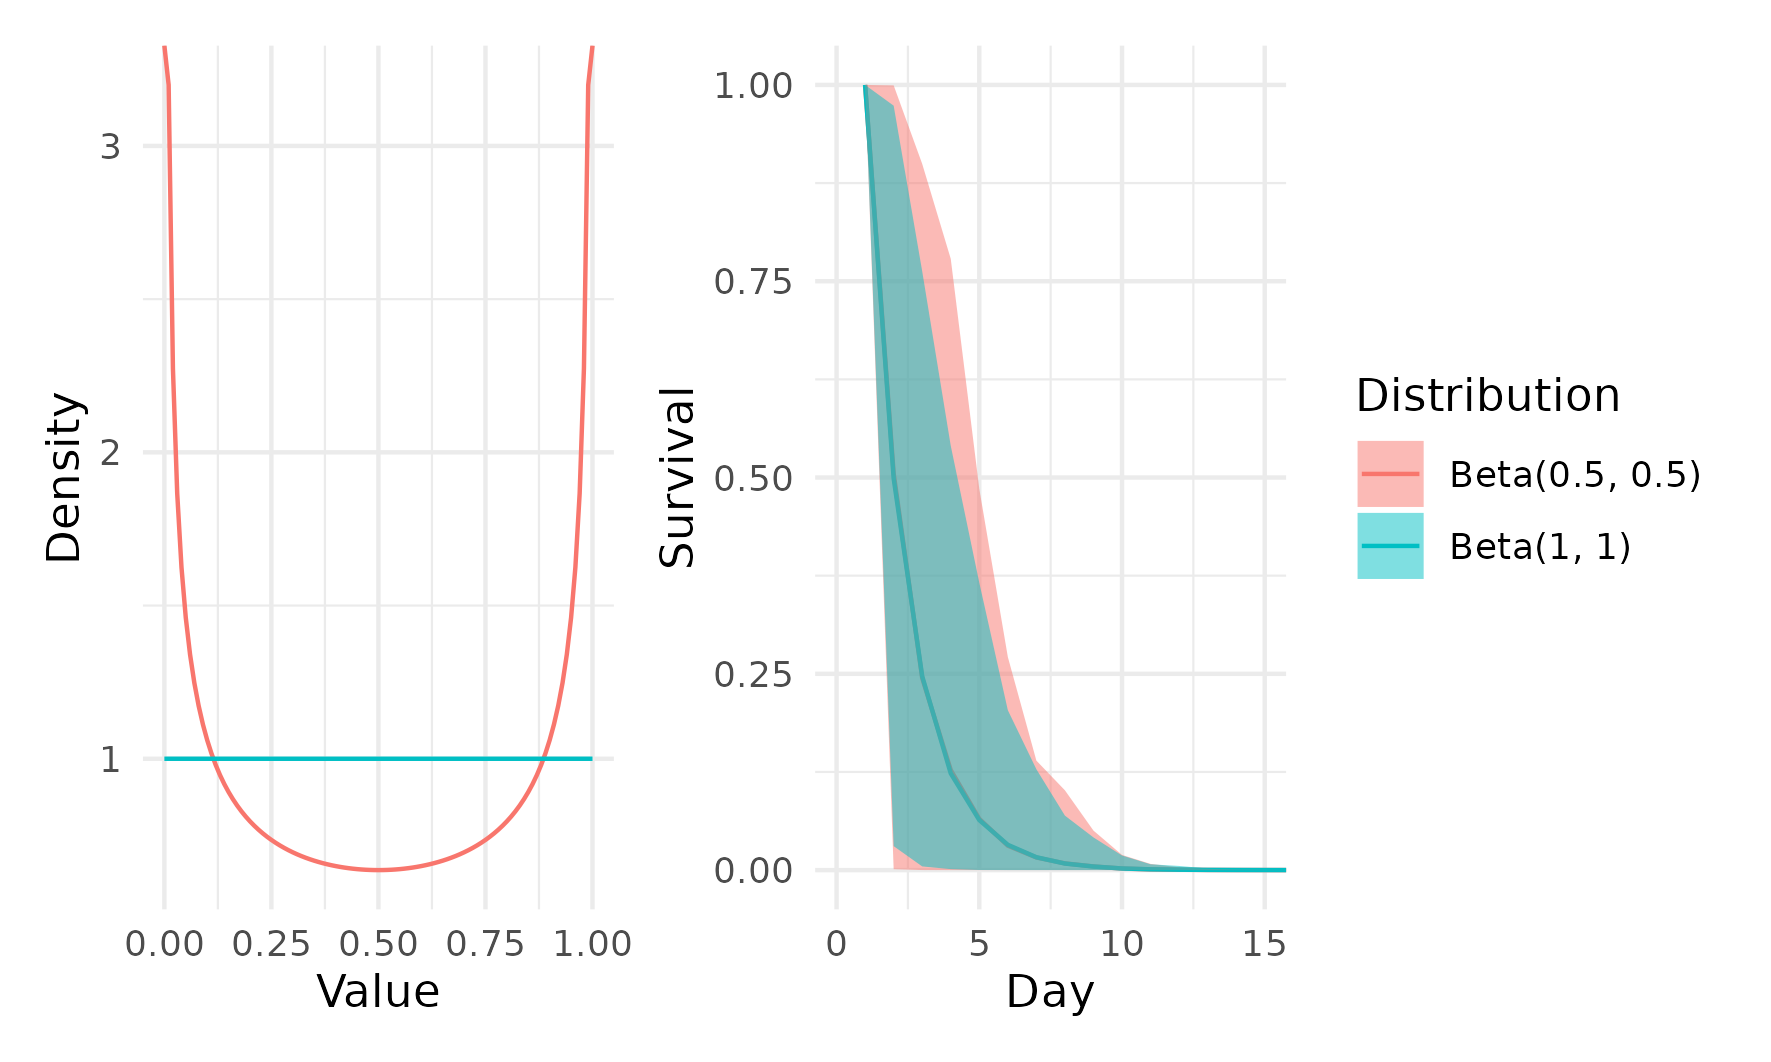
\includegraphics{cis-perfect-testing/flat-prior}
  \caption[Uninformative priors for the hazard]{The density of Beta(1, 1) flat prior and Beta(0.5, 0.5) uninformative priors (left) with the prior predictive survival time (right). The implied prior on the survival time is very short when using either prior on the hazard at each time. \label{perf-test:fig:flat-prior}}
\end{figure}

Instead, I propose a weakly informative (or vague) prior Beta(0.1, 1.9), which has mean 0.05 and minimal information.
The amount of information in a Beta distribution is related to the sum of its parameters.
Here, the sum equals 2, the same as the flat prior case.
The central 95\% probability mass of Beta(0.1, 1.9) is 0.00--0.47.
The central estimate, of 0.05, is in line with previous estimates that the median duration is in the range 15--20 days~\autocite{cevikShedding}.
This prior gives a very vague prior predictive distribution on the survival time (see \cref{perf-test:fig:vague-prior}).
\begin{figure}
  \centering 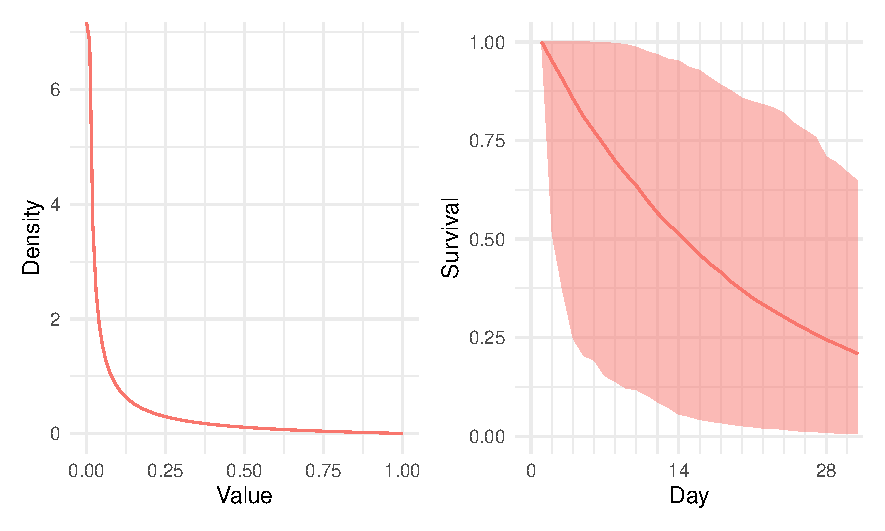
\includegraphics{cis-perfect-testing/vague-prior}
  \caption[Vague prior for the hazard]{The density of Beta(0.1, 1.9) vague prior (left) and the prior predictive survival time (right). The prior predictive survival time is very vague using a Beta(0.1, 1.9) prior. Note the different x-axis to \cref{perf-test:fig:flat-prior}. \label{perf-test:fig:vague-prior}}
\end{figure}


\subsection{Smoothing priors}

Smoothing priors encode the biological consideration that the hazard should not vary significantly from day-to-day.
It is the Bayesian equivalent of a penalised likelihood, used frequently in the non-parametric frequentist setting~\autocite[e.g.][]{bacchettiNonparametric}.
Many possible forms of smoothing priors exist, including splines, Gaussian Processes, and random walks.
I use a second-order random walk (RW2) because it is simple and produces sensible prior predictive distributions.

RW2 prior encodes that the hazard should be linearly changing with some random changes at each time step.
Specifically, the difference on the logit scale between $\lambda_t$ to $\lambda_{t+1}$ is the difference between $\lambda_{t-1}$ and $\lambda_t$ plus some Normally-distributed noise.
Formally:
\begin{align}
  \logit\lambda_{t+1}
  &= \logit\lambda_t + (\logit\lambda_t - \logit\lambda_{t-1}) + \sigma \epsilon_t &\text{for $t \geq 2$} \\
  &= 2\logit\lambda_t - \logit\lambda_{t-1} + \sigma \epsilon_t \\
  \epsilon_t &\dist \N(0, 1) &\text{for $t \geq 2$}  \\
  \logit\lambda_2 &= \logit\lambda_1 + \epsilon_1 \\\
  \epsilon_1 &\dist \N(\mu_{\epsilon_1}, \sigma_{\epsilon_1}^2) \\
  \logit \lambda_1 &\dist \N(\mu_{\lambda_1}, \sigma_{\lambda_1}^2) \\
  \sigma &\dist \Exponential(1/\mu_\sigma).
\end{align}
The hyperparameters $\mu_{\lambda_1}$ and $\sigma_{\lambda_1}$ specify the prior on the hazard at time 1; $\mu_{\epsilon_1}$ and $\sigma_{\epsilon_1}$ the prior on the initial gradient; and $\mu_\sigma$ the smoothness of the random walk.
I use $\mu_{\lambda_1} = -17.5$, $\sigma_{\lambda_1} = 6$, $\mu_\epsilon = 1.09$, $\sigma_\epsilon = 0.03$, and $\mu_\epsilon = 0.1$ based on the analysis in \cref{E-ATACCC} (see \cref{perf-test:fig:rw2-prior}).
\begin{figure}
  \centering 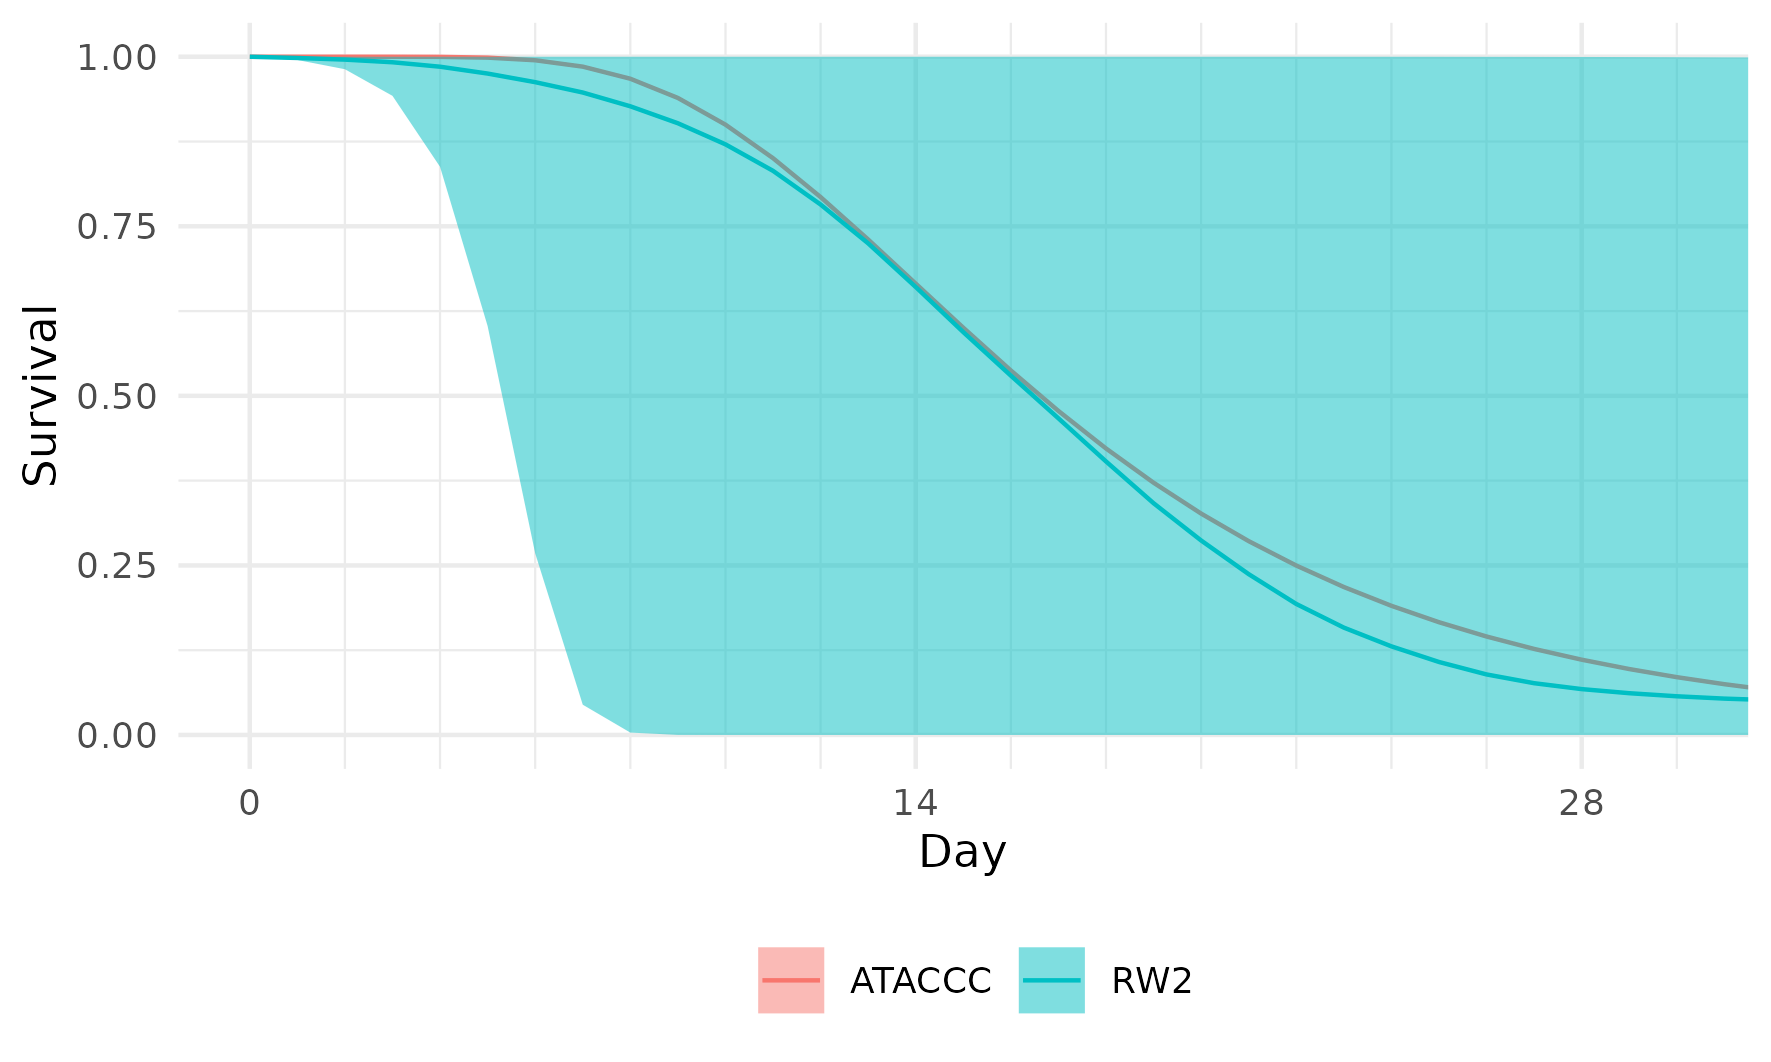
\includegraphics{cis-perfect-testing/rw2-prior}
  \caption[RW2 prior for the hazard]{The of prior predictive distribution (mean and 95\% central interval) for the RW2 prior specified in the main text. The posterior mean estimate using ATACCC data in \cref{E-ATACCC} are shown for comparison. \label{perf-test:fig:rw2-prior}}
\end{figure}

\subsection{Model combination priors} \label{perf-test:sec:informative-priors}

The information from \cref{E-ATACCC} can be incorporated through the prior.
This is desirable because the ATACCC study frequently sampled individuals early in the infection.
Therefore, \cref{E-ATACCC}'s estimate of the survival distribution in the early infection period should be reliable.
In the later infection period, the ATACCC study has fewer observations and hence the estimates are less reliable.
CIS can inform the posterior in this region.

When constructing the prior, two aspects need consideration.
Firstly, the model structure from \cref{E-ATACCC} leads to positive correlation in the posterior estimates of the hazard, which should be propagated into this analysis.
That is, the prior used in this analysis cannot be independent across the hazards.
Secondly, the uncertainty in the estimates from \cref{E-ATACCC} should be increased for this analysis.
The additional uncertainty is because the \cref{E-ATACCC} analysis extrapolates beyond the data using strong model assumptions (see \cref{E-ATACCC:sec:discussion}).
%Furthermore, there are differences in the study design and laboratories used between the two studies (see \cref{E-intro:sec:studies}) which may mean that results do not generalise between the studies.
I form the prior for the combination in two steps.

I first approximate the \cref{E-ATACCC} posterior estimate of the hazard as a multivariate normal on the logit scale.
This can be viewed as an approximation of Markov melding~\autocite{goudieJoining}.
Using a multivariate normal, as opposed to multiple univariate distribution, ensures that the correlation between the hazards is preserved.
The logit transformation maps from the $[0, 1]$ interval to the full real line.
To estimate the parameters of the multivariate normal, I use the method of moments.
The approximation is very good (see \cref{perf-test:fig:approximate-ATACCC-hazard} and \cref{perf-test:fig:approximate-ATACCC-survival}).
\begin{figure}
  \thisfloatpagestyle{empty}
  \vspace{-2.5cm}
  \makebox[\textwidth][c]{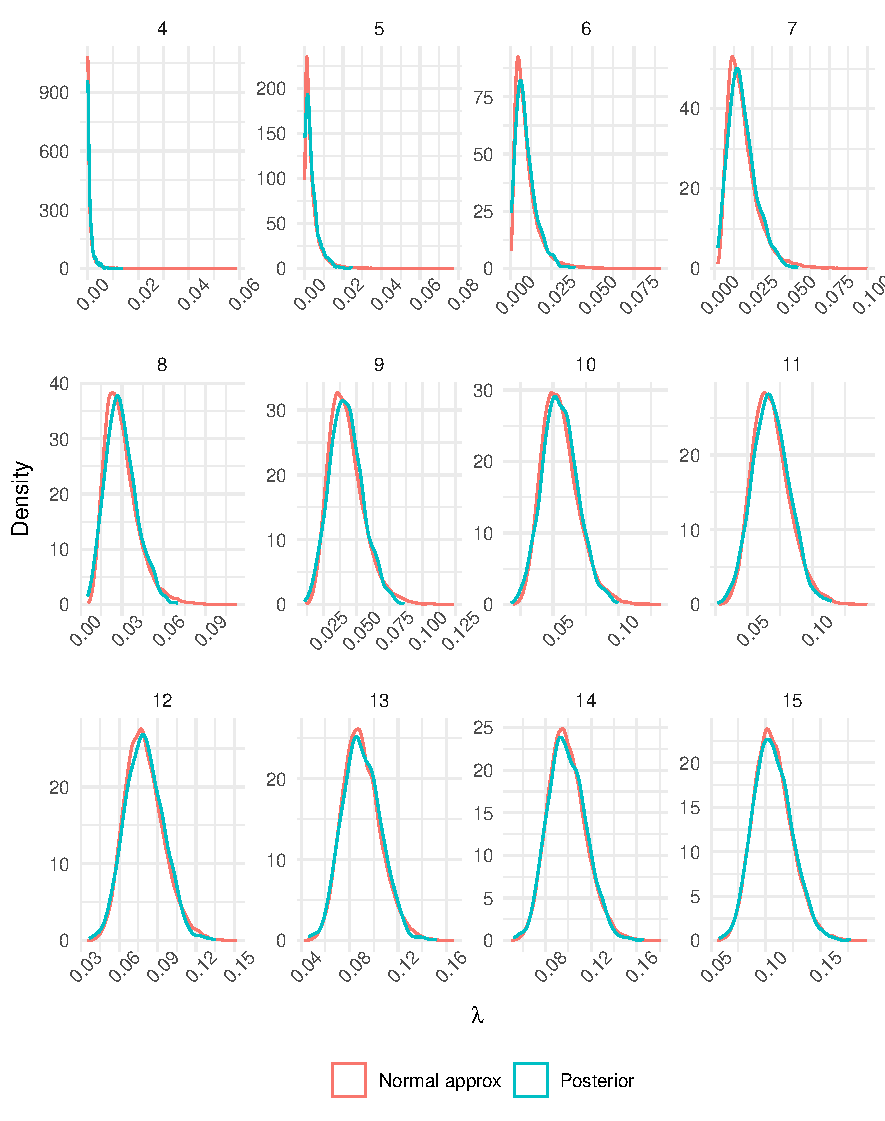
\includegraphics[width=.9\paperwidth]{cis-perfect-testing/ataccc-approximation-hazard}}
  \caption[Approximating the ATACCC posterior hazard as a logit-normal]{Comparison of the posterior estimate of the hazard from \cref{E-ATACCC} and its approximation with a logit-normal distribution (kernel density estimate smoothed) for the first 15 hazards. \label{perf-test:fig:approximate-ATACCC-hazard}}
\end{figure}
\begin{figure}
  \centering 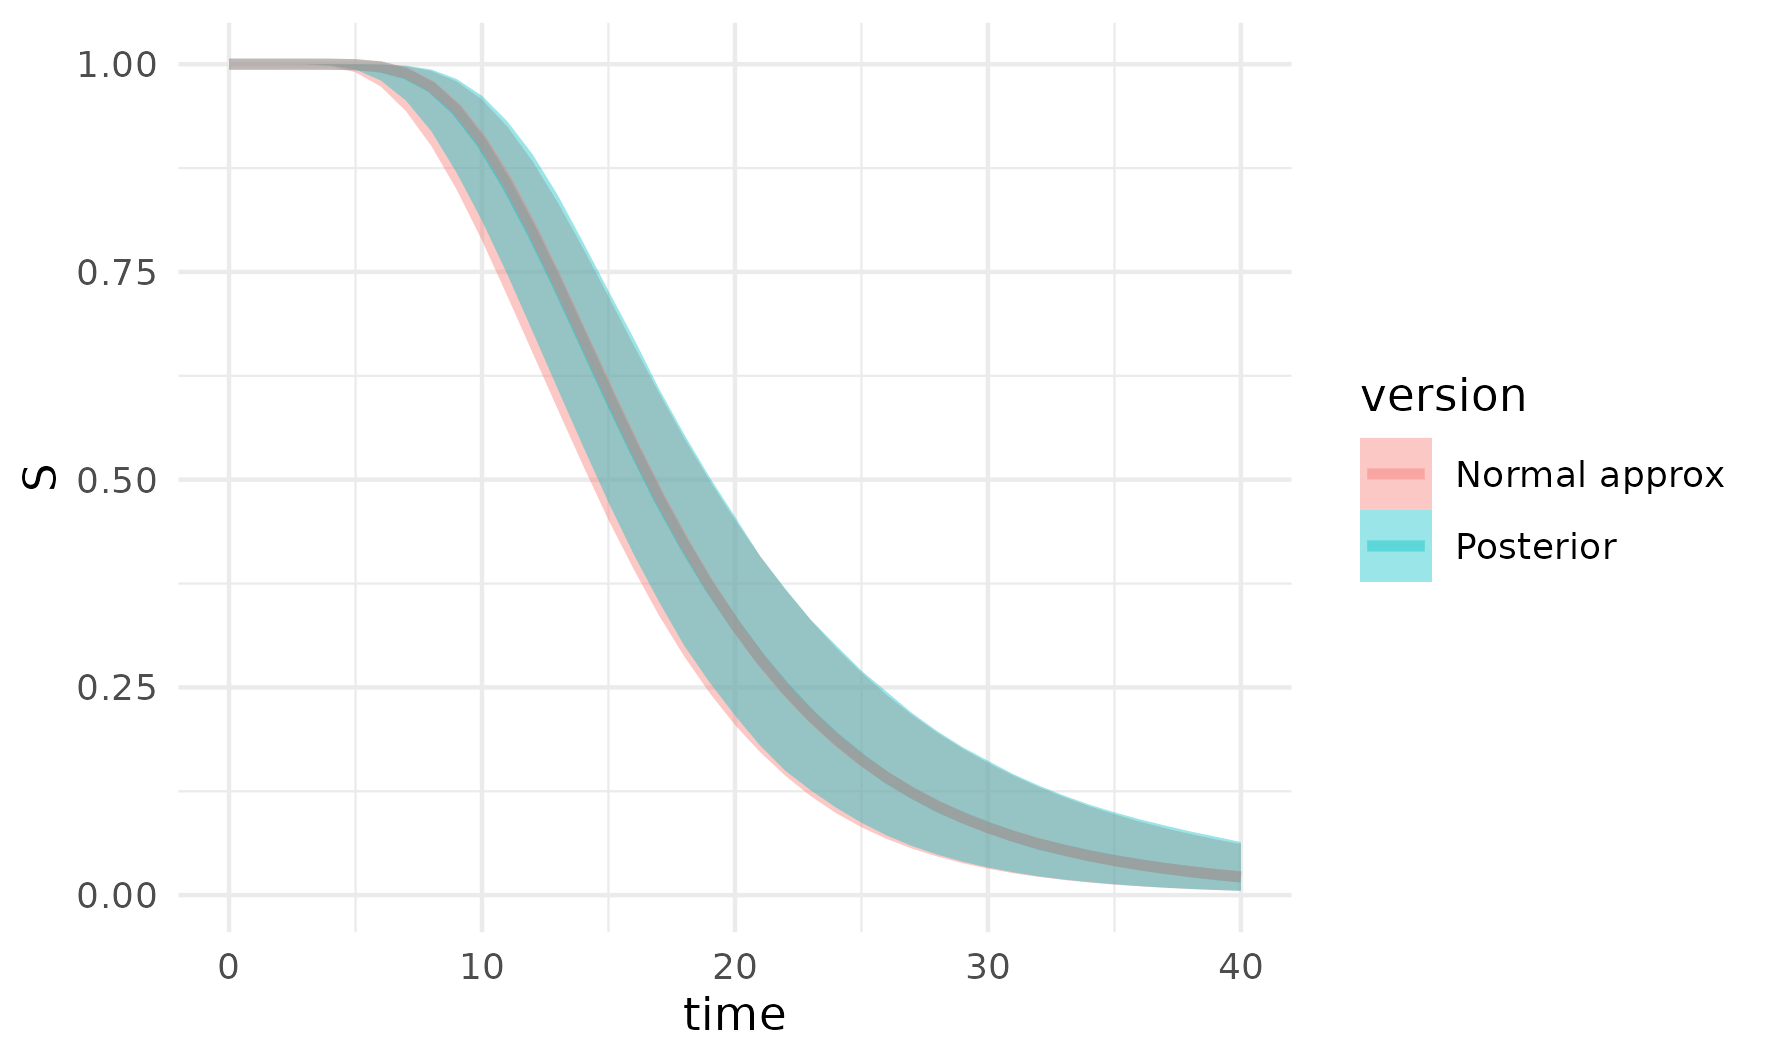
\includegraphics{cis-perfect-testing/ataccc-approximation-survival}
  \caption[Approximating the ATACCC posterior survival as a logit-normal]{Comparison of the posterior estimate of the survival from \cref{E-ATACCC} and its approximation with a logit-normal distribution (median and central 95\% interval). The survival is a function of all the hazards up until that point, therefore the correlation between the hazards must be well-approximated to have these agree. \label{perf-test:fig:approximate-ATACCC-survival}}
\end{figure}

Having approximated the estimate as a multivariate normal, I add additional uncertainty using a discrete Beta process.
The discrete Beta process prior generalises the form of prior used in \cref{perf-test:sec:independent-priors} by allowing the central estimate of the hazard to vary over time~\autocite{ibrahimBayesian,sunStatisticala}.
It is:
\begin{align}
  \lambda_t &\sim \text{Beta}(\alpha_t, \beta_t) &t = 1, 2, \dots \\
  \alpha_t &= k_t h_t + \alpha_0 \\
  \beta_t &= k_t (1 - h_t) + \beta_0
\end{align}
where $k_t$, $\alpha_0$, and $\beta_0$ are hyperparameters; and $h_t$ is a point estimate of the hazard at time $t$ from ATACCC.
An intuition for what this distribution represents can be gained from a conjugate model for $\lambda_t$ with a beta prior and a binomial likelihood.
If $\lambda_t$ is given the prior distribution $\text{Beta}(\alpha_0, \beta_0)$, and we then have $k_t$ observations with $k_t h_t$ successes, then the posterior distribution for $\lambda_t$ is $\text{Beta}(\alpha_t, \beta_t)$ (as defined above).

$k_t$ reflects the subjective belief that the estimates from \cref{E-ATACCC} are very reliable in the early infection period but unreliable by day 30.
The equation for $k_t$ is below and shown in \cref{perf-test:fig:kt}.
\begin{align}
k_t = \begin{cases}
  \expit(-0.4 * (t - 20)) &\text{for $t \leq 39$} \\
  0 &t > 39
\end{cases}
\end{align}
where $\expit(x) = 1 / (1 + \exp(-x))$.

\begin{figure}
  \centering 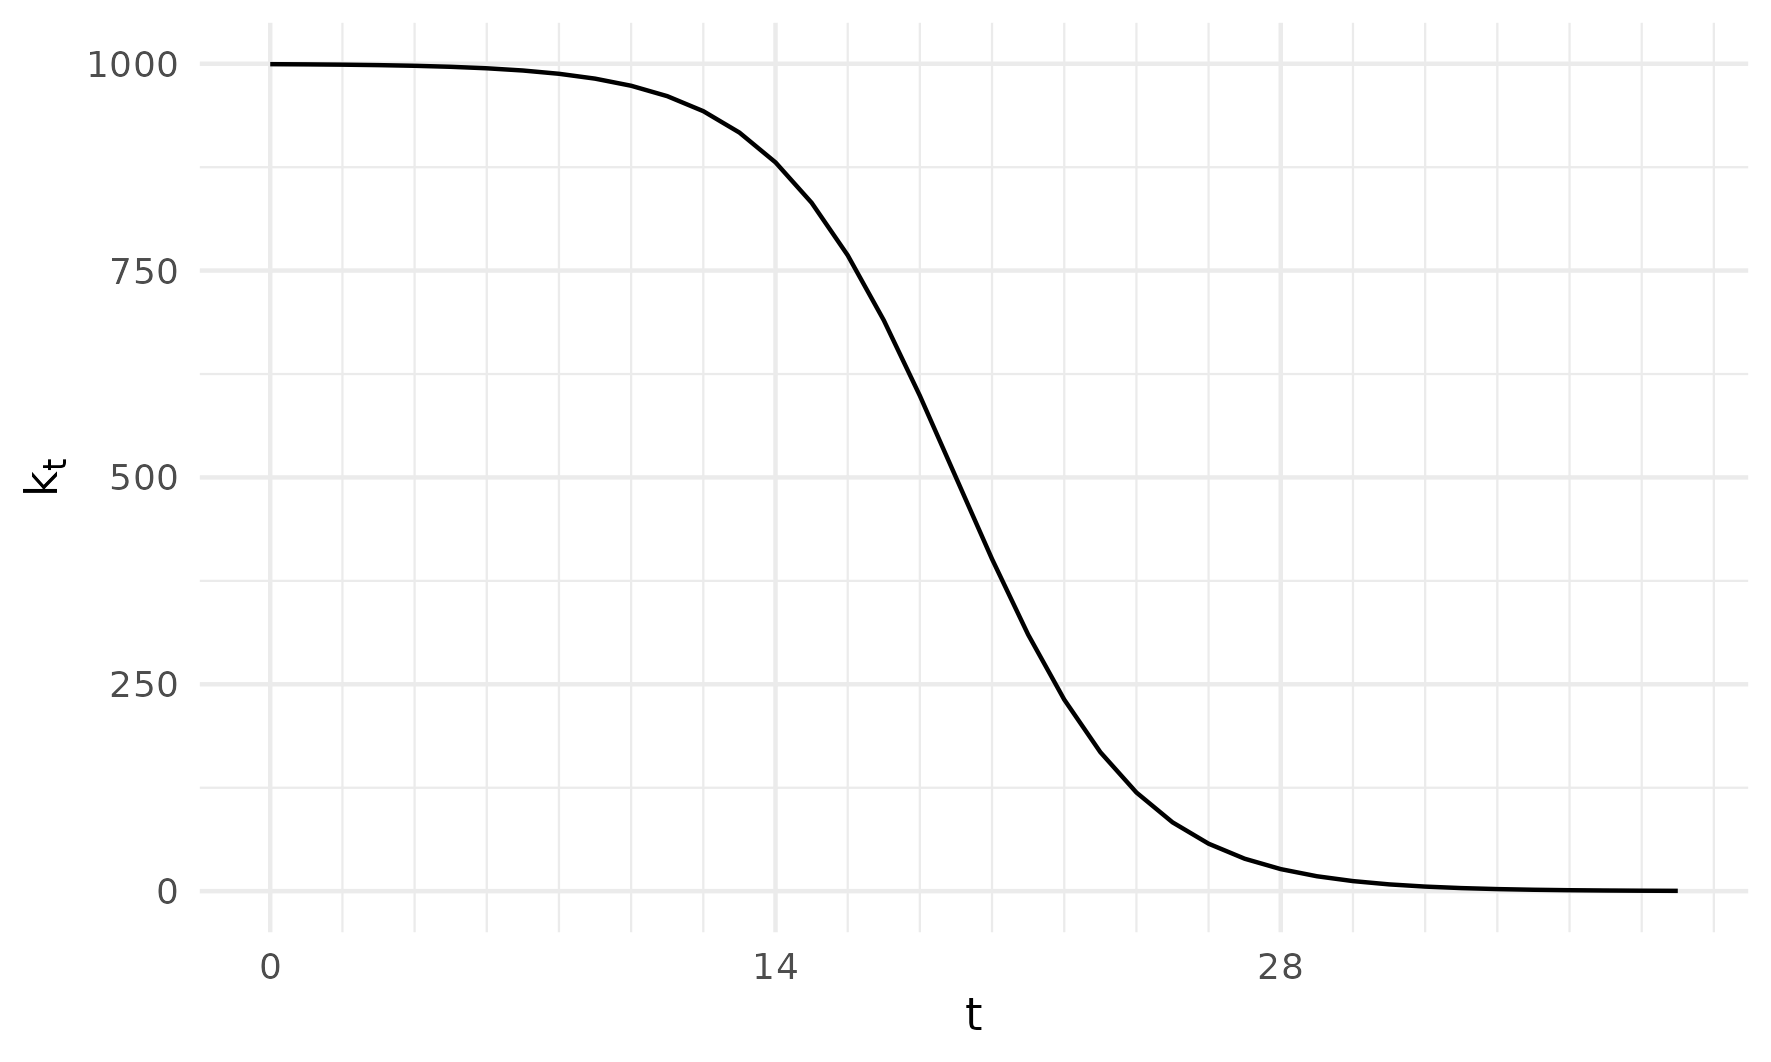
\includegraphics{cis-perfect-testing/kt-prior}
  \caption{Function used for $k_t$. \label{perf-test:fig:kt}}
\end{figure}

\section{Simulation study} \label{perf-test:sec:simulation-study}

\subsection{Setup}

I simulate a dataset of detected episodes that has the same characteristics as that in the CIS by the following procedure.
\begin{enumerate}
    \item Extract the test schedules for each individual who had at least one test during the period of interest.
    \item Draw an episode start time, $b_{j(i)}$ for each individual uniformly at random between 2nd July 2020 (100 days before the period where a detected episode would be included) and 6th December 2020 (the end of this period).
    \item Draw a duration of episode for each individual, $d_i$, based on the distribution described below. Then calculate the end of their infection episode, $e_{j(i)} = b_{j(i)} + d_i - 1$.
    \item Simulate the test results based on the test schedule, $b_{j(i)}$, and $e_{j(i)}$. Tests between $b_{j(i)}$ and $e_{j(i)}$ (inclusive) are positive, all other tests are negative.
    \item Discard episodes where there are no positive tests (\ie undetected episodes) and then apply the same inclusions/exclusions as in \cref{perf-test:sec:problem}.
    \item Of these remaining episodes, sample 4,800 to match the sample size of the true dataset. This is needed because in step 2 the entire cohort was infected, while in the real study only a (unknown) portion is infected.
    \item For this final set of episodes, calculate $(l_j^{(b)}, r_j^{b}, l_j^{(e)}, r_j^{(e)})$ by taking the day after the last negative prior to any positives, the first positive, the last positive, and the day before the negative following the last positive respectively.
\end{enumerate}

To generate the durations, an assumption is required for the distribution of the duration of positivity.
I base this assumption on the estimate from \cref{E-ATACCC} with an inflated tail to represent what is seen within CIS.
The tail is modified based on an unpublished analysis of CIS data~\citePersonalComms{A.\ Sarah Walker}.
Walker uses survival analysis to estimate the duration from CIS data.
The initiating event is assumed known as the time the episode was detected.
The final event is assumed interval-censored between the time of the final positive test and the subsequent negative test, or right-censored if a negative test has not yet been observed.
A flexible, spline-based form is assumed for the baseline survival function~\autocite{roystonSTPM,roystonFlexible} with covariates introduced via proportional odds.
By not accounting for either the undetected infections or the interval censoring of the initiating event, this analysis has competing biases which makes them hard to interpret~\autocite{cisMethodsONS}.

% \todo[inline]{The following seems important to justify why we can't just use these estimates but is also basically an aside}
% We know of two biases introduced from this analysis.
% \enquote{There is a bias in estimating the clearance distribution because the analysis used to estimate how long a person stays positive only starts from their first positive test.
% Since (most) people will have become positive on an earlier day, this will bias the clearance curves downwards (making the estimates too short).
% However, there is another bias due to the survey missing positive episodes entirely if they are short.
% This means that our dataset has fewer short positive episodes than in the population as a whole, and that the sample used to run the survival analysis is biased towards people with longer positive episodes.
% This will bias the clearance curves upwards (making the estimates too long).}~\autocite{cisMethodsONS}.

To form the duration distribution used in the simulation, we combine the two estimates.
The first 30 days of the distribution is proportional to the ATACCC estimate, with the rest proportional to this CIS-based estimates.
% The CIS-based estimates are shifted 3 days in order to make this smooth; this counteracts the above bias of missing the start of the infection (for times above 30 days, the other bias, missing short infections, is negligible). ERR... I'M NOT DOING THIS ANYMORE OH NO!!
Denote by $f_A(t)$ the distribution function estimated in \cref{E-ATACCC} and $f_C(t)$ that from the CIS-based estimates just derived.
Then define:
$$
f_S'(t) = \begin{cases}
	f_A(t) &t \leq 30 \\
	f_C(t) &t > 30
\end{cases}
$$
Then the distribution used in the simulation is the normalised version of this: $f_S(t) = f'_S(t)/\sum_i f_S'(i)$.
These curves and the combined curve are compared in \cref{perf-test:fig:duration-dist}.
Individual $i$'s duration of positivity, $D_i$, is then an independent draw from this distribution.
\begin{figure}
  \centering 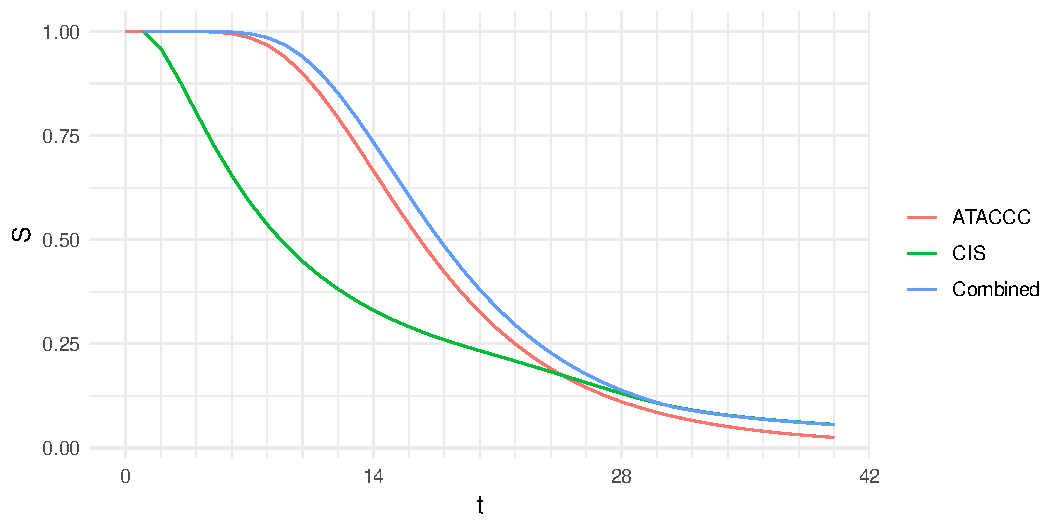
\includegraphics{cis-perfect-testing/input-duration-dists}
  \caption[Comparison of duration distributions]{Comparison of the duration distribution used for the simulation. ATACCC is the posterior mean from \cref{E-ATACCC}'s analysis, CIS is Sarah Walker's analysis, and Combined is the combination of these used for the simulation. See main text for details of each analysis. \label{perf-test:fig:duration-dist}}
\end{figure}

\subsection{Implementation}

Simulation was performed in R~4.2.0~\autocite{R-4-2-0} using tidyverse~2.0.0~\autocite{tidyverse} and targets~1.1.3~\autocite{targetsPackage}.

Inference was implemented in Stan via RStan~2.21.8~\autocite{rstan2-21-8} using default settings.
Convergence was assessed using Rhat and ESS as described in \cref{E-inc-prev:sec:MCMC}, and all runs checked for divergent transitions.

The prior on the total number of infections was centred on the true value with a dispersion parameter of 1.
This meant that the prior was very diffuse.


\subsection{Results} \label{perf-test:sec:results}

Repeating the simulation showed negligible variation in the results (not shown).
This is caused by the large sample size (4800 detected infections).
Therefore, only results from a single simulation are shown and discussed.

All analyses converged.
Rhat were below 1.01, all parameters had an effective sample size of 1000, and there were no divergent transitions.

The true value of the survival function was generally well recovered (see \cref{perf-test:fig:survival-results}).
This was especially true for the first 30 days of the distribution.

The second-order random walk prior performed worst.
It showed oversmoothing, especially in the later parts of the distribution.
It smooths towards a linearly changing hazard; here, linearly decreasing (see \cref{perf-test:fig:hazard-results}).
This means that the survival function decreases slower than an exponential distribution in the tail.

The informative and vague independent priors performed similarly.
The informative prior had tighter credible intervals, as expected.
This prior was centred on the correct value for the initial part of the distribution.
Therefore, the narrow credible intervals are unsurprising.
For hazards after day 40, the informative and vague priors are the same.
Therefore, the posterior distributions are almost identical.
There remains a difference because the hazard estimates are partially dependent on earlier estimates.

\begin{figure}
  \centering 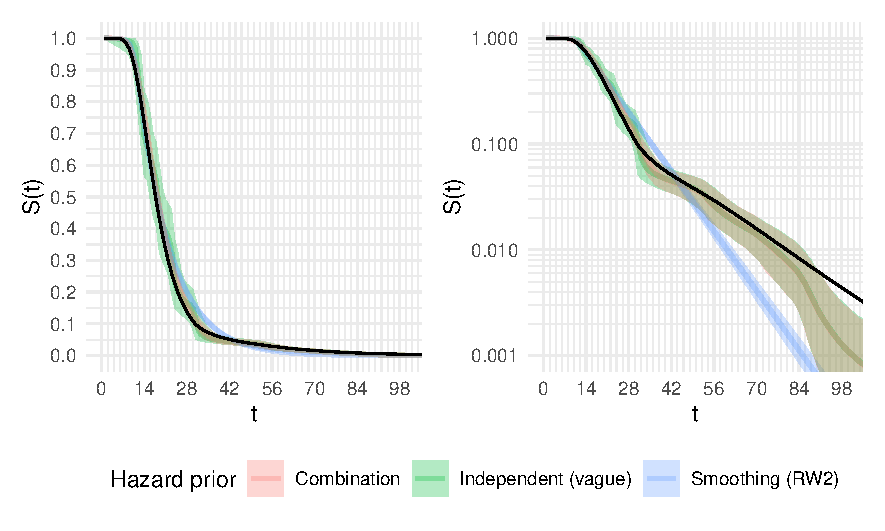
\includegraphics{cis-perfect-testing/survival-results}
  \caption[Comparison of survival function estimates under different priors]{Comparison of the posterior estimate of the survival distribution (pointwise median and 95\% CrI) when using different priors on the hazard. Results using each of the three different priors discussed in \cref{perf-test:sec:parameters-priors} are shown. y-axis has either natural (left) or log (right) scale. Only showing first 100 days of the distribution. \label{perf-test:fig:survival-results}}
\end{figure}

\begin{figure}
  \centering 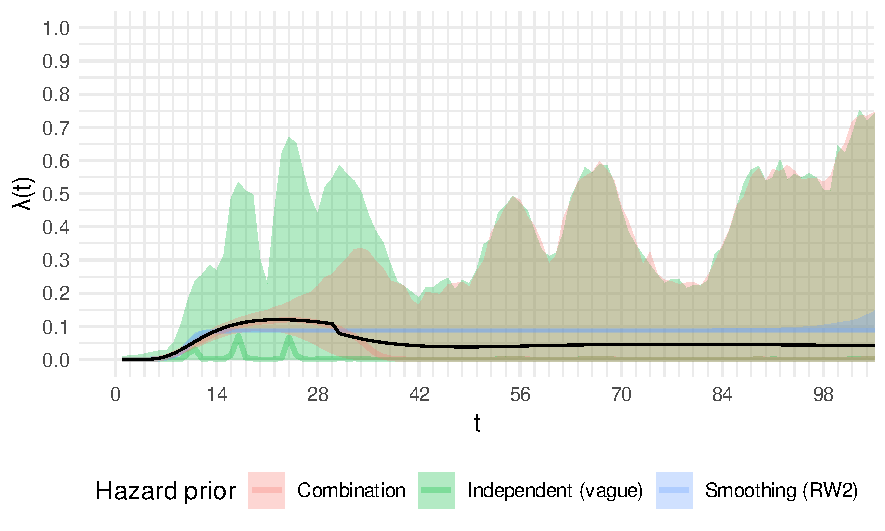
\includegraphics{cis-perfect-testing/hazard-results}
  \caption[Comparison of hazard estimates under different priors]{Comparison of the posterior estimate of the hazard (pointwise median and 95\% CrI) when using different priors on the hazard. Results using each of the three different priors discussed in \cref{perf-test:sec:parameters-priors} are shown. \label{perf-test:fig:hazard-results}}
\end{figure}

\section{Discussion} \label{perf-test:sec:discussion}

This chapter shows that the model I propose can recover the true survival function well.
However, the problem becomes substantially harder if false negatives are present, as we shall see in the next chapter.
Unfortunately, false negatives do occur in the CIS data.

Reasonable choices of the prior for the hazard are vague (although not flat) or informative.
A smoothing prior performed poorly, although that may be influenced by the choice of hyperparameters.
Reducing the amount of smoothing or type of smoothing may help.
More flexible smoothers, such as a Gaussian Process for additional flexibility and smoothing and different time-scales~\autocite{saulGaussian}.

Various extensions could be worth exploring.
Most importantly, covariates (\eg age, immunity from vaccination and/or previous infection, or variant) could be included.
Immunity in particular affects the duration substantially, although age and variant may also make a contribution~\autocite{hakkiOnset,russellWithinhost}.
Covariates can be included with a variety of models, the simplest being a proportional hazards model.
A major challenge here is that the calculation of $p_t$ is greatly complicated, because it is no longer linear in the survival function.

The prior would likely be more important if the number of detected infections was smaller.
Therefore, exploring its impact could be important for future surveys.
A particular application would be estimation in the early stages of an epidemic of a novel pathogen.
Here, little would be known about the pathogen, but gathering information with robust estimates of uncertainty is important to inform the response.

I have assumed a prior of constant incidence and that incidence is independent between individuals.
Prevalence in the CIS data was approximately constant over the period of interest (see \cref{E-biology-data:sec:positivity-results}).
A sensitivity analysis, where an epidemic in exponential growth or decline was simulated (not shown), showed minimal impact on survival estimates.
An incorrect assumption of constant incidence can lead to biased estimates~\autocite{degruttolaAnalysis}.
Therefore, the assumption could be important in other contexts, especially if the incidence is changing rapidly.

I have developed a flexible simulation and inference framework for this type of analysis.
This framework could be used to simulate alternate study designs.
The design of CIS was created on a very short timescale in March 2020, in response to the pandemic's rapid spread.
Therefore, it is likely that there are more efficient designs.
These could be more cost-effective.
Improved cost-effectiveness could allow more rapid response to potential pandemics because the threshold for policy-makers to approve the study would be lower.
A long-term, preparatory effort to develop a more efficient design in preparation of a future pandemic would be worthwhile.

Other useful preparatory work would be developing reasonable priors.
These could be based on seasonal viruses that are of the same family as those likely to cause future pandemics.
For example, seasonal influenzas and coronaviruses.
These would allow analyses such as those performed in these chapters to be performed more rapidly in a future pandemic scenario.

\section{Conclusion} \label{perf-test:sec:conclusion}
This chapter has shown the feasibility of estimating the survival function from a study with a CIS-like testing schedule.
While the infrequent testing schedule is not ideal, appropriate modelling can recover the true survival function well.

\ifSubfilesClassLoaded{
  \listoftodos
}{}
\end{document}